\documentclass[a4paper]{article}
%
\usepackage{geometry}
\usepackage{tikz}
\usetikzlibrary{3d}
\usetikzlibrary{patterns}
\usepackage{ifthen}
\usetikzlibrary{backgrounds,fit}
\usetikzlibrary{calc}

\geometry{margin=2cm}

% Define colors
\definecolor{red}{RGB}{255,0,0}
\definecolor{green}{RGB}{0,255,0}
\definecolor{blue}{RGB}{0,0,255}
\definecolor{yellow}{RGB}{255,255,0}
\definecolor{white}{RGB}{255,255,255}
\definecolor{orange}{RGB}{255,165,0}
\definecolor{pale}{RGB}{170,170,170}

%%%%%%%%%%%%%%%%%%%%%%%%%%%%%%%%%%%%%%%%%%%%%%%%%%%%%%%%%%%%%%%%%%%%%%%%%%%%%
% X=-1(Left)..1(Right)
\newcommand{\cubeLeftFace}[1]{
  \begin{scope}[canvas is yz plane at x=0]
    % Left face
    \ifthenelse{\not\equal{#1}{-1}}{\tikzset{left/.style={fill=pale}}}{}
    \path[draw=black,left] (0,0) rectangle ++(1,1);
  \end{scope}
}
\newcommand{\cubeRightFace}[1]{
  \begin{scope}[canvas is yz plane at x=1]
    \ifthenelse{\not\equal{#1}{+1}}{\tikzset{right/.style={fill=pale}}}{}
    \path[draw=black,right] (0,0) rectangle ++(1,1);
  \end{scope}
}

% Y=-1(Bottom)..+1(Top)
\newcommand{\cubeBottomFace}[1]{
  \begin{scope}[canvas is xz plane at y=0]
    \ifthenelse{\not\equal{#1}{-1}}{\tikzset{bottom/.style={fill=pale}}}{}
    \path[draw=black,bottom] (0,0) rectangle ++(1,1);
  \end{scope}
}
\newcommand{\cubeTopFace}[1]{
  \begin{scope}[canvas is xz plane at y=1]
    \ifthenelse{\not\equal{#1}{+1}}{\tikzset{top/.style={fill=pale}}}{}
    \path[draw=black,top] (0,0) rectangle ++(1,1);
  \end{scope}
}

% Z=0(Front)..-2(Back)
\newcommand{\cubeFrontFace}[1]{
      \begin{scope}[canvas is xy plane at z=0]
        % Front face
        \ifthenelse{\not\equal{#1}{0}}{\tikzset{front/.style={fill=pale}}}{}
        \path[draw=black,front] (0,0) rectangle ++(1,1);
      \end{scope}
}
\newcommand{\cubeBackFace}[1]{
      \begin{scope}[canvas is xy plane at z=-1]
        \ifthenelse{\not\equal{#1}{-2}}{\tikzset{back/.style={fill=pale}}}{}
        \path[draw=black,back] (0,0) rectangle ++(1,1);
      \end{scope}
}

%%%%%%%%%%%%%%%%%%%%%%%%%%%%%%%%%%%%%%%%%%%%%%%%%%%%%%%%%%%%%%%%%%%%%%%%%%%%%

\newcommand{\drawCubicleSouthEast}[4][X]{
  \ifthenelse{\equal{#1}{X}}{
    \begin{scope}[shift={(#2,#3,#4)}]
      %\cubeBackFace{#4}
      %\cubeTopFace{#3}
      %\cubeLeftFace{#2}
      \cubeBottomFace{#3}
      \cubeRightFace{#2}
      \cubeFrontFace{#4}
    \end{scope}
}{}
}

\newcommand{\drawCubicleNorthEast}[4][X]{
  \ifthenelse{\equal{#1}{X}}{
    \begin{scope}[shift={(#2,#3,#4)}]
      %\cubeBackFace{#4}
      %\cubeTopFace{#3}
      %\cubeLeftFace{#2}
      \cubeTopFace{#3}
      \cubeRightFace{#2}
      \cubeFrontFace{#4}
    \end{scope}
}{}
}

\newcommand{\drawCubicleNorthWest}[4][X]{
  \ifthenelse{\equal{#1}{X}}{
    \begin{scope}[shift={(#2,#3,#4)}]
      %\cubeBackFace{#4}
      %\cubeBottomFace{#3}
      %\cubeRightFace{#2}
      \cubeTopFace{#3}
      \cubeLeftFace{#2}
      \cubeFrontFace{#4}
    \end{scope}
}{}
}

%%%%%%%%%%%%%%%%%%%%%%%%%%%%%%%%%%%%%%%%%%%%%%%%%%%%%%%%%%%%%%%%%%%%%%%%%%%%%

% Define the function to draw a single cubicle
\newcommand{\drawcubicle}[5][X]{
  \ifthenelse{\equal{#1}{X}}{
  \begin{scope}[shift={#2}]
    % Front face
    \begin{scope}[canvas is xy plane at z=0]
      \path[draw=black,#3] (0,0) rectangle (1,1);
    \end{scope}
    % Top face
    \begin{scope}[canvas is xz plane at y=1]
      \path[draw=black,#4] (0,0) rectangle (1,1);
    \end{scope}
    % Right face
    \begin{scope}[canvas is yz plane at x=1]
      \path[draw=black,#5] (0,0) rectangle (1,1);
    \end{scope}
  \end{scope}
}{}
}

\newcommand{\cubeCanvas}{
  % Draw the Rubik's Cube
  \foreach \x in {0,1,2} {
    \foreach \y in {0,1,2} {
      \foreach \z in {2,1,0} {
        \drawcubicle{(\x,\y,\z)}{draw=white}{draw=white}{draw=white}
      }
    }
  }
}


\pgfdeclarepatternformonly{upwards arrows}
  {\pgfpointorigin}{\pgfpoint{1cm}{0.3cm}}{\pgfpoint{1cm}{0.3cm}}
  {
  % Draw the triangles
  \pgfpathmoveto{\pgfpoint{0}{0}}
  \pgfpathlineto{\pgfpoint{0.25cm}{0}}
  \pgfpathlineto{\pgfpoint{0.5cm}{0.15cm}}
  \pgfpathlineto{\pgfpoint{0.75cm}{0}}
  \pgfpathlineto{\pgfpoint{1cm}{0}}
  \pgfpathlineto{\pgfpoint{0.5cm}{0.3cm}}
  \pgfpathlineto{\pgfpoint{0}{0}}
  \pgfpathclose
  \pgfusepath{fill}
}

\tikzset{inner/.style={fill=gray!50!white,draw=black}}



\title{Alain's Rubik's Methods}
\author{Alain Lehmann}

\begin{document}

\maketitle
%\tableofcontents

\raggedright
\section{Mnemonics}
\centering

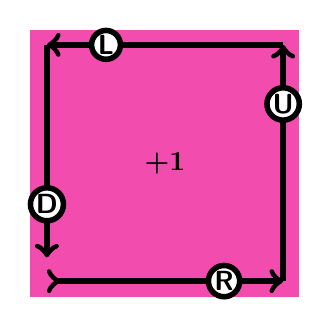
\begin{tikzpicture}
\tikzset{arrowlabel/.style={pos=0.75,draw=black,fill=white,circle,inner sep=0.5pt,font=\sffamily\bfseries}}
\tikzset{ultrathick/.style={line width=2}}
\begin{scope}[local bounding box=BB,scale=1.5]
  \draw (0,0) coordinate(X);
  \draw[>->,ultrathick] (X) -- ++(2,0) node[arrowlabel]{R} coordinate(X);
  \draw[->,ultrathick] (X) -- ++(0,2) node[arrowlabel]{U} coordinate(X);
  \draw[->,ultrathick] (X) -- ++(-2,0) node[arrowlabel]{L} coordinate(X);
  \draw[->,ultrathick] (X) -- ++(0,-1.8) node[arrowlabel]{D} coordinate(X);
  \draw (1,1) node{\bf +1};
  \begin{pgfonlayer}{background}
    \fill[magenta,opacity=0.7] (BB.north west) rectangle (BB.south east);
  \end{pgfonlayer}
\end{scope}
\end{tikzpicture}%
%
\begin{tikzpicture}
\tikzset{top/.style={fill=green}}
\tikzset{bottom/.style={fill=blue}}
\tikzset{right/.style={fill=red}}
\tikzset{left/.style={fill=orange}}
\tikzset{front/.style={fill=yellow}}
\tikzset{back/.style={fill=white}}
\tikzset{ultrathick/.style={line width=2}}
\tikzset{arrowlabel/.style={pos=0.75,draw=black,fill=white,circle,inner sep=0.5pt,font=\sffamily\bfseries}}
\input{special_base.tex}
\end{tikzpicture}%
%
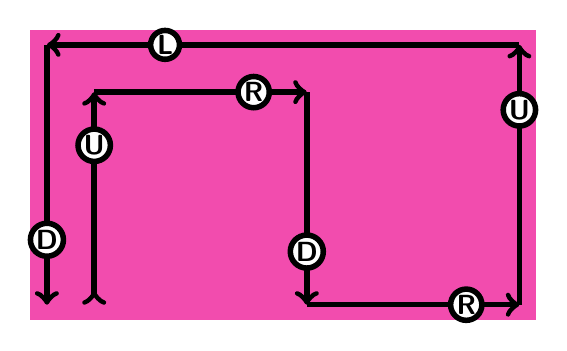
\begin{tikzpicture}
  \tikzset{ultrathick/.style={line width=2}}
  \tikzset{arrowlabel/.style={pos=0.75,draw=black,fill=white,circle,inner sep=0.5pt,font=\sffamily\bfseries}}
  \tikzset{rotarrow/.style={->, shorten >=4, shorten <=4, line width=2}}
  \tikzset{movarrow/.style={->, line width=2}}

  \begin{scope}[scale=3.0,local bounding box=BB]
  \path (0.1,0) coordinate (x);
    \draw[movarrow,>->] (x) -- ++(0,+0.9) coordinate(x) node[arrowlabel]{U};
    \draw[movarrow] (x) -- ++(+0.9,+0) coordinate(x) node[arrowlabel]{R};
    \draw[movarrow] (x) -- ++(0,-0.9) coordinate(x) node[arrowlabel]{D};
    \draw[movarrow] (x) -- ++(+0.9,0) coordinate(x) node[arrowlabel]{R};
    \draw[movarrow] (x) -- ++(0,+1.1) coordinate(x) node[arrowlabel]{U};
    \draw[movarrow] (x) -- ++(-2,0) coordinate(x) node[arrowlabel]{L};
    \draw[movarrow] (x) -- ++(0,-1.1) coordinate(x) node[arrowlabel]{D};
    \begin{pgfonlayer}{background}
      \fill[magenta,opacity=0.7] (BB.north west) rectangle (BB.south east);
    \end{pgfonlayer}
  \end{scope}
\end{tikzpicture}

\raggedright
\section{Solution process}
\centering

\tikzset{front/.style={fill=red}}
\tikzset{top/.style={fill=white}}
\tikzset{right/.style={fill=blue}}
\input{00_initial.tex}%
\input{01_top_cross.tex}%
\input{02_top_layer.tex}%

\tikzset{front/.style={fill=blue}}
\tikzset{top/.style={fill=yellow}}
\tikzset{right/.style={fill=red}}
\input{03_top_layer_upside_down.tex}%
\begin{tikzpicture}[z={(0.5cm,0.5cm)}]
  \cubeCanvas
%%%% BOTTOM
\drawcubicle[X]{(0,0,2)}{inner}{inner}{inner} % 1
\drawcubicle[X]{(1,0,2)}{inner}{inner}{inner} %   2
\drawcubicle[X]{(2,0,2)}{inner}{inner}{right} %     3
\drawcubicle[X]{(0,0,1)}{inner}{inner}{inner} % 4
\drawcubicle[X]{(1,0,1)}{inner}{inner}{inner} %   5
\drawcubicle[X]{(2,0,1)}{inner}{inner}{right} %     6
\drawcubicle[X]{(0,0,0)}{front}{inner}{inner} % 7
\drawcubicle[X]{(1,0,0)}{front}{inner}{inner} %   8
\drawcubicle[_]{(2,0,0)}{front}{inner}{right} %     9
%%
%%%% MIDDLE
\drawcubicle[X]{(0,1,2)}{inner}{inner}{inner} % 1
\drawcubicle[X]{(1,1,2)}{inner}{inner}{inner} %   2
\drawcubicle[X]{(2,1,2)}{inner}{inner}{right} %     3
\drawcubicle[X]{(0,1,1)}{inner}{inner}{inner} % 4
\drawcubicle[X]{(1,1,1)}{inner}{inner}{inner} %   5
\drawcubicle[X]{(2,1,1)}{inner}{inner}{right} %     6
\drawcubicle[X]{(0,1,0)}{front}{inner}{inner} % 7
\drawcubicle[X]{(1,1,0)}{front}{inner}{inner} %   8
\drawcubicle[_]{(2,1,0)}{front}{inner}{right} %     9
%%
%%%% TOP
\drawcubicle[_]{(0,2,2)}{inner}{top}{inner} % 1
\drawcubicle[_]{(1,2,2)}{inner}{top}{inner} %   2
\drawcubicle[_]{(2,2,2)}{inner}{top}{right} %     3
\drawcubicle[_]{(0,2,1)}{inner}{top}{inner} % 4
\drawcubicle[X]{(1,2,1)}{inner}{top}{inner} %   5
\drawcubicle[_]{(2,2,1)}{inner}{top}{right} %     6
\drawcubicle[_]{(0,2,0)}{front}{top}{inner} % 7
\drawcubicle[_]{(1,2,0)}{front}{top}{inner} %   8
\drawcubicle[_]{(2,2,0)}{front}{top}{right} %     9
%%
\end{tikzpicture}
%
\input{05_top_cross_almost.tex}%

\input{06_top_cross.tex}%
\tikzset{front/.style={fill=red}}
\tikzset{top/.style={fill=green}}
\tikzset{right/.style={fill=white}}
\input{07_top_cross_rotated.tex}%
\input{08_final.tex}%

\raggedright
\section{Top Cross Rotation \& Solving Corners}
\centering

\tikzset{top/.style={fill=green}}
\tikzset{bottom/.style={fill=blue}}
\tikzset{right/.style={fill=red}}
\tikzset{left/.style={fill=orange}}
\tikzset{front/.style={fill=yellow}}
\tikzset{back/.style={fill=white}}


\begin{tikzpicture}
  \begin{scope}[z={(-0.5cm,+0.5cm)}]
    \drawCubicleNorthWest[X]{+1}{+1}{2}
    \drawCubicleNorthWest[X]{+0}{+1}{2}
    \drawCubicleNorthWest[X]{-1}{-1}{2}
    \drawCubicleNorthWest[X]{-1}{+0}{2}
    \drawCubicleNorthWest[X]{-1}{+1}{2}
    %
    \drawCubicleNorthWest[X]{-1}{-1}{1}
    \drawCubicleNorthWest[X]{-1}{-0}{1}
    \drawCubicleNorthWest[X]{+1}{+1}{1}
    \drawCubicleNorthWest[X]{+0}{+1}{1}
    \drawCubicleNorthWest[X]{-1}{+1}{1}
    %
    \drawCubicleNorthWest[X]{-0}{-1}{0}
    \drawCubicleNorthWest[X]{+1}{-0}{0}
    \drawCubicleNorthWest[_]{+1}{+1}{0}
    \drawCubicleNorthWest[X]{+0}{+0}{0}
    \drawCubicleNorthWest[X]{-1}{+0}{0}
    \drawCubicleNorthWest[X]{-0}{+1}{0}
  \end{scope}%
  \begin{scope}[z={(+0.5cm,-0.5cm)}]
    %% BACK
    \drawCubicleSouthEast[X]{-1}{-1}{2}
    \drawCubicleSouthEast[X]{-0}{-0}{2}
    \drawCubicleSouthEast[X]{+1}{+1}{2}
    %
    \drawCubicleSouthEast[X]{+0}{-1}{2}
    \drawCubicleSouthEast[X]{+1}{-0}{2}
    %
    \drawCubicleSouthEast[_]{+1}{-1}{2}

    %% MIDDLE
    \drawCubicleSouthEast[X]{-1}{-1}{1}
    \drawCubicleSouthEast[X]{-0}{-0}{1}
    \drawCubicleSouthEast[X]{+1}{+1}{1}
    %
    \drawCubicleSouthEast[X]{+0}{-1}{1}
    \drawCubicleSouthEast[X]{+1}{-0}{1}
    %
    \drawCubicleSouthEast[X]{+1}{-1}{1}

    %% FRONT
    \drawCubicleSouthEast[X]{-1}{-0}{0}
    \drawCubicleSouthEast[X]{-0}{+1}{0}
    %
    \drawCubicleSouthEast[_]{-1}{-1}{0}
    \drawCubicleSouthEast[X]{+0}{-0}{0}
    \drawCubicleSouthEast[_]{+1}{+1}{0}
    %
    \drawCubicleSouthEast[X]{-0}{-1}{0}
    \drawCubicleSouthEast[X]{+1}{-0}{0}
    %
    \drawCubicleSouthEast[_]{+1}{-1}{0}
  \end{scope}%
\end{tikzpicture}%


\begin{tikzpicture}
\begin{scope}
  [x={(0.9cm,-0.1cm)},y={(0,0.9cm)},z={(0.6cm,0.4cm)}]
% BACK
\drawCubicleNorthEast[X]{-1}{-1}{2}
\drawCubicleNorthEast[X]{-1}{-0}{2}
\drawCubicleNorthEast[X]{-0}{-1}{2}
\drawCubicleNorthEast[X]{-1}{+1}{2}
\drawCubicleNorthEast[X]{-0}{+0}{2}
\drawCubicleNorthEast[X]{+1}{-1}{2}
\drawCubicleNorthEast[X]{-0}{+1}{2}
\drawCubicleNorthEast[X]{+1}{-0}{2}
\drawCubicleNorthEast[X]{+1}{+1}{2}
%MIDDLE
\drawCubicleNorthEast[X]{-1}{-1}{1}
\drawCubicleNorthEast[X]{-1}{-0}{1}
\drawCubicleNorthEast[X]{-0}{-1}{1}
\drawCubicleNorthEast[X]{-1}{+1}{1}
\drawCubicleNorthEast[X]{-0}{+0}{1}
\drawCubicleNorthEast[X]{+1}{-1}{1}
\drawCubicleNorthEast[X]{-0}{+1}{1}
\drawCubicleNorthEast[X]{+1}{-0}{1}
\drawCubicleNorthEast[X]{+1}{+1}{1}
% FRONT
\drawCubicleNorthEast[X]{-1}{-1}{0}
\drawCubicleNorthEast[X]{-1}{-0}{0}
\drawCubicleNorthEast[X]{-0}{-1}{0}
\drawCubicleNorthEast[X]{-1}{+1}{0}
\drawCubicleNorthEast[X]{-0}{+0}{0}
\drawCubicleNorthEast[X]{+1}{-1}{0}
\drawCubicleNorthEast[X]{-0}{+1}{0}
\drawCubicleNorthEast[X]{+1}{-0}{0}
\drawCubicleNorthEast[X]{+1}{+1}{0}
%% FRONT
  \begin{scope}[canvas is xz plane at y=2.0]
    \draw[fill=black, fill opacity=0.5,even odd rule]
      (0.5,1.5) circle (1.4)
      (0.5,1.5) circle (1.0)
    ;
  \end{scope}
  \begin{scope}[canvas is yz plane at x=2.0]
    \draw[fill=black, fill opacity=0.5,even odd rule]
      (0.5,1.5) circle (1.4)
      (0.5,1.5) circle (1.0)
    ;
  \end{scope}
  \tikzset{arrowlabel/.style={draw=black,fill=white,circle,inner sep=0.5pt}}
  \draw[->,very thick] (-0.5,+1.5+0.2,0) -- ++(2.0,0,0) node[pos=0.8,arrowlabel]{1};
  \draw[->,very thick] (+1.5+0.2,-0.5,0) -- ++(0,2.0,0) node[pos=0.8,arrowlabel]{2};
  \draw[<-,very thick] (-0.5,+1.5-0.2,0) -- ++(2.0,0,0) node[pos=0.2,arrowlabel]{3};
  \draw[<-,very thick] (+1.5-0.2,-0.5,0) -- ++(0,2.0,0) node[pos=0.2,arrowlabel]{4};
\end{scope}

  \foreach \i in {0, 60, 120, 180, 240, 300} {
    \path[->] (1.0,0.5) -- ++(\i:6) node{\i} coordinate(A);
    \begin{scope}[shift={(A)},local bounding box=a]
      \begin{scope}[z={(-0.5cm,+0.5cm)}]
      \drawCubicleNorthWest[X]{-1}{+1}{0}
      \end{scope}
      \begin{scope}[z={(+0.5cm,-0.5cm)}]
      \drawCubicleSouthEast[X]{+1}{-1}{0}
      \end{scope}
    \end{scope}
    \begin{pgfonlayer}{background}
      \fill[yellow,opacity=0.3] (a.south west) rectangle (a.north east);
    \end{pgfonlayer}
  }
\end{tikzpicture}%


\end{document}
